\newpage
\section{Question 3}
	\subsection*{The Iterated Closed Loop Algorithm}
	\noindent
	\newline
	By modifying the given code pieces, we will implement an Iterated Closed Loop algorithm to estimate the position of a vehicle as it moves through its surroundings.\newline All code pieces, original and modified, can be found in the Appendix.
		\subsubsection{Part A - Implementing the ICP}
		\newline
		By modifying the given showICP.m file, we will exam the resultant ICP features generated for a single data set. The set in question is frame 500, and we will use frame 520 as our initial 'guess'.\newline Firstly, using the default variables of a grid size of 0.005, and a maximum iterative loop of 40, we can generate the following graph:\newline
			\begin{figure}[position = here]
				\begin{centering}
					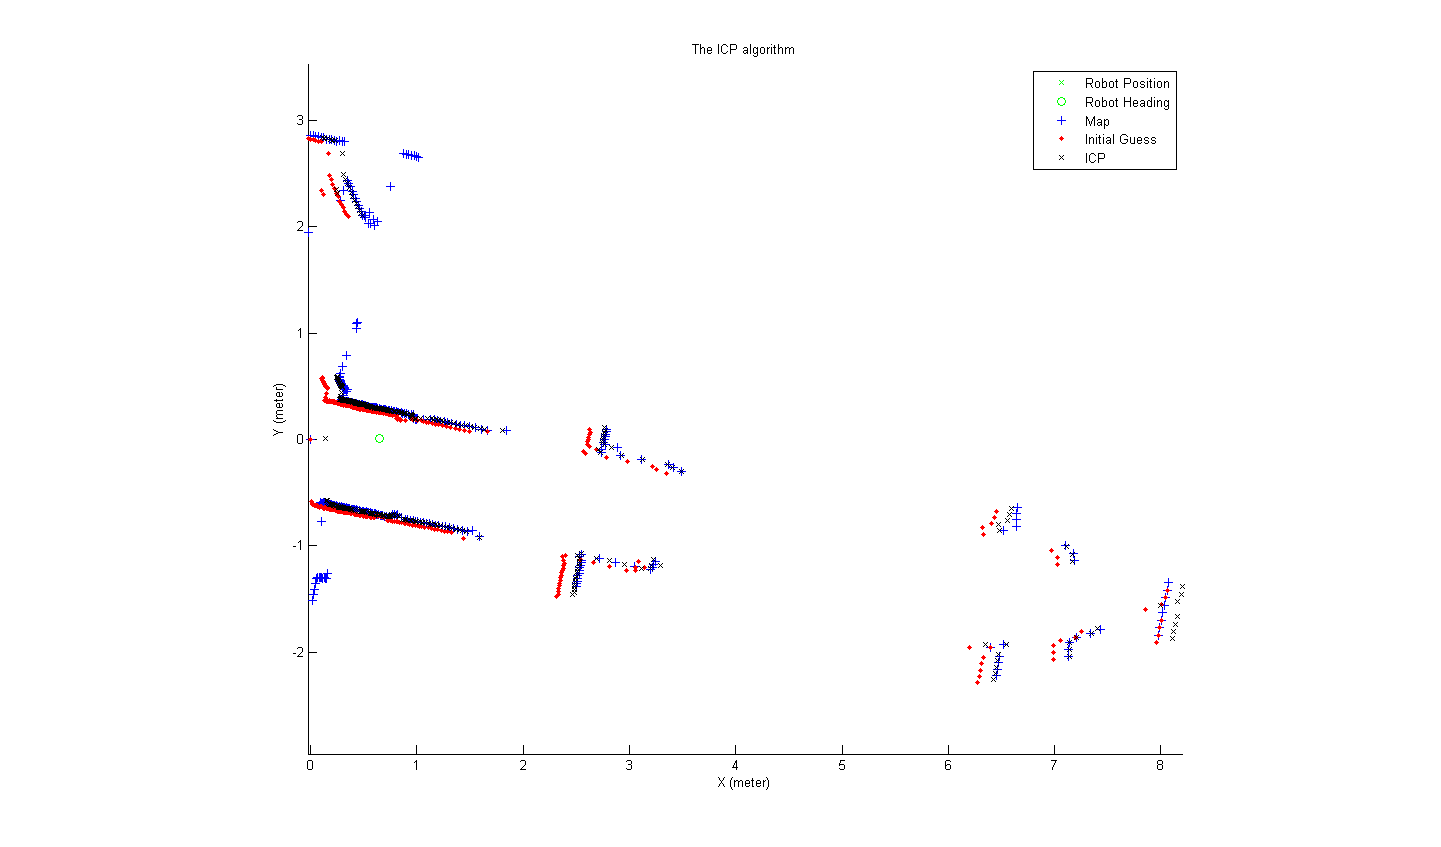
\includegraphics[scale=0.5]{q3a_1_1}\\
					\caption[\textit{RPYAxes}]{ICP estimate for maximum iterations of 40 and grid size of 0.005}
				\end{centering}
			\end{figure}
		\newline
		We will now examine the effect of modifying some of the variables of the ICPv4.m algorithm.\newline Firstly we will look at changing the grid size. For a smaller grid size of 0.001 we obtain the following graph:\newline
		
			\begin{figure}[position = here]
				\begin{centering}
					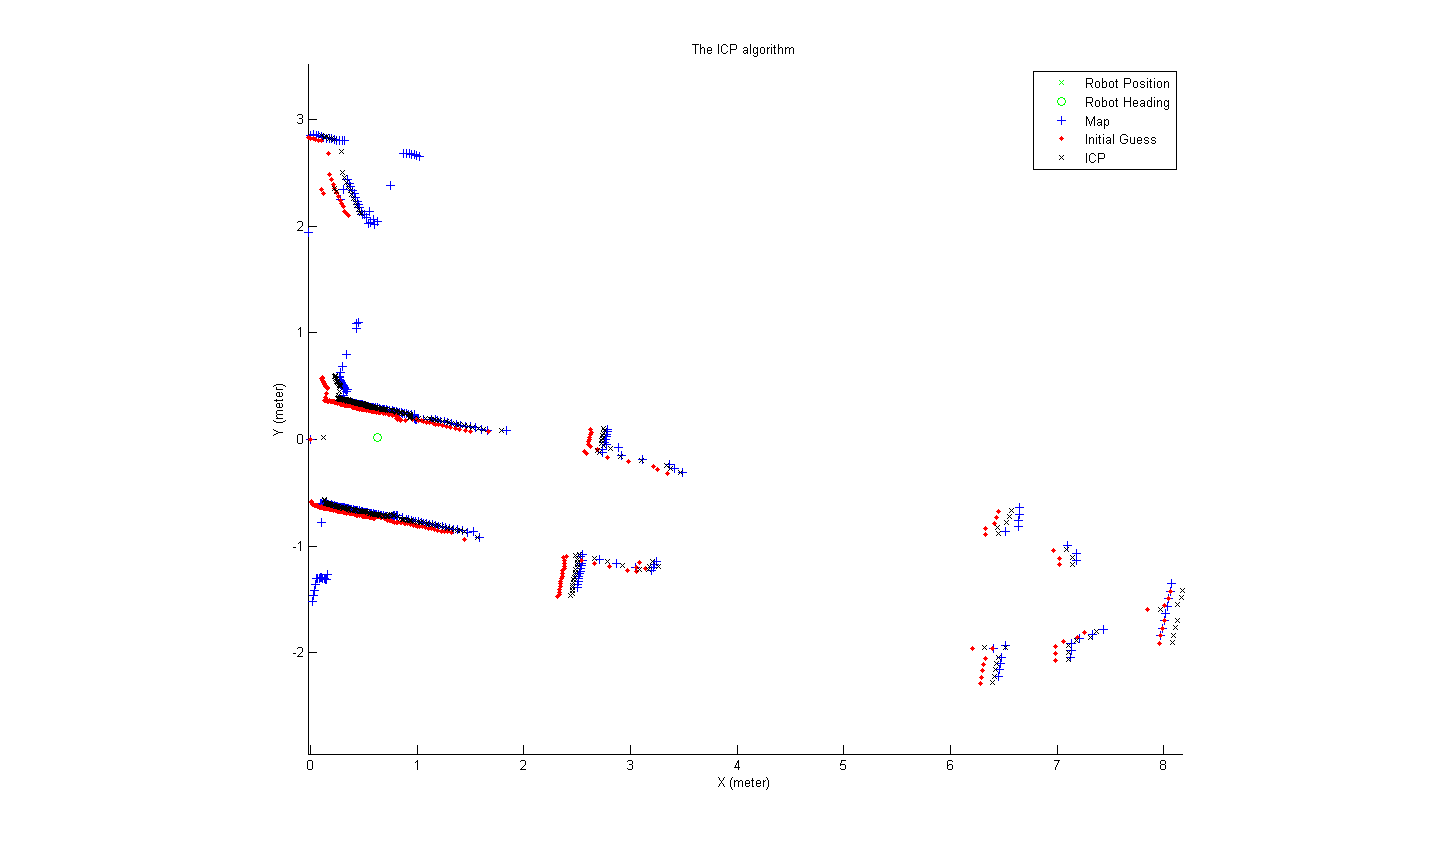
\includegraphics[scale=0.5]{q3a_1_2}\\
					\caption[\textit{RPYAxes}]{ICP estimate for maximum iterations of 40 and grid size of 0.001}
				\end{centering}
			\end{figure}
			
		\newline	
		\pagebreak	
		Next, for a grid size of 0.1:\newline
		
			\begin{figure}[position = here]
				\begin{centering}
					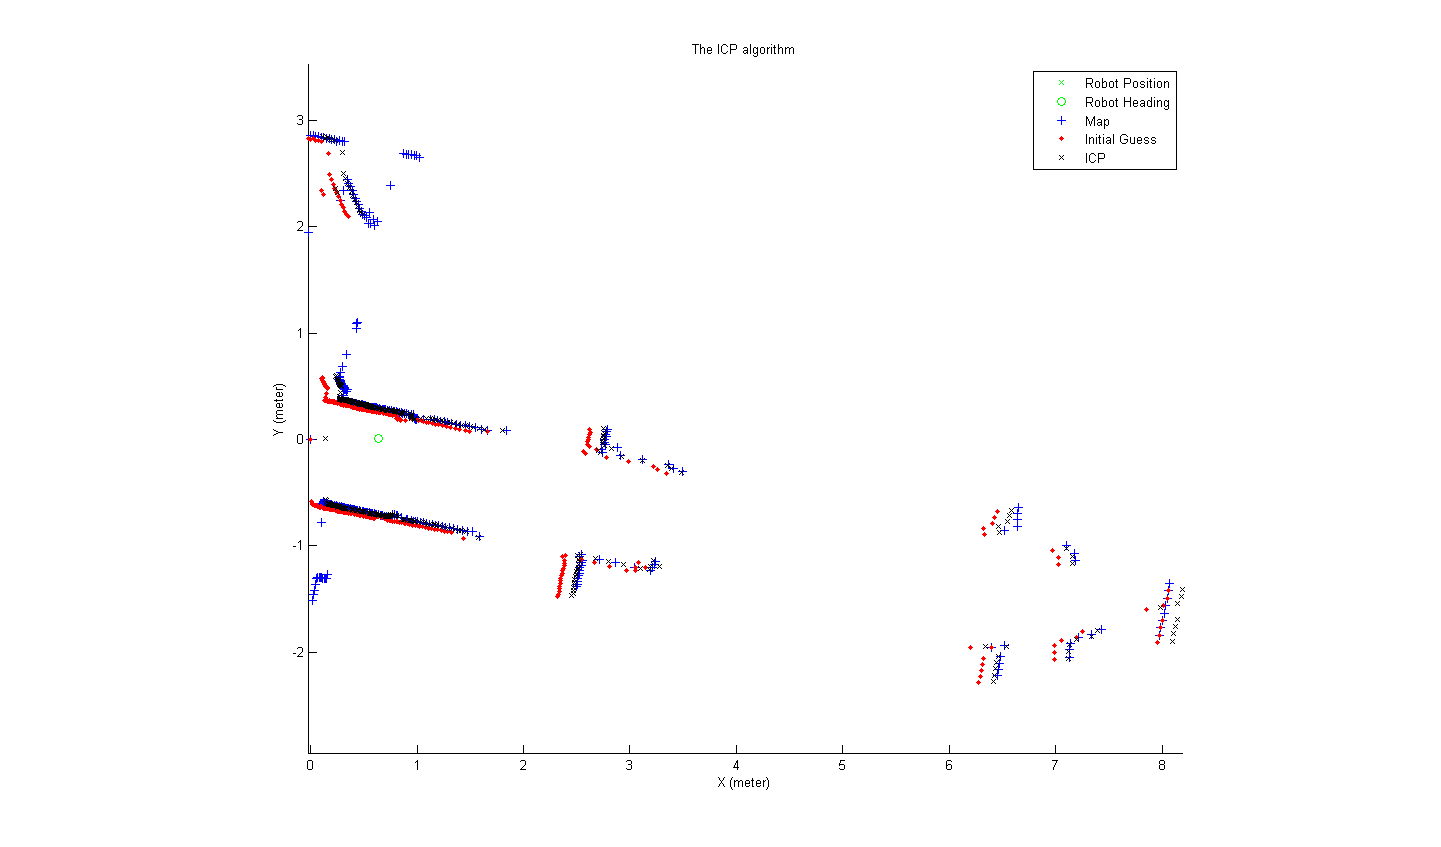
\includegraphics[scale=0.5]{q3a_1_3}\\
					\caption[\textit{RPYAxes}]{ICP estimate for maximum iterations of 40 and grid size of 0.005}
				\end{centering}
			\end{figure}
			
		\newline As can be seen, changing the grid size has little effect on the overall ICP . \newline It does, however, have an affect on the number of collision points detected. For a grid size of 0.005, 188 points collide. For 0.001, 32 points collide, and for 0.01, 252 points collide. This is expected - an increase in in the grid size means a large sample section, with a greater likelihood of multiple points landing in a grid.\newline \newline
		Checking for matching pairs reveals an interesting point - for all tested values for grid size, the number of matching points is the same - 362. Also of worthy note, despite a maximum number of iterations of 40, no more than 9 iterations are used. Changing the maximum number of iterations to 10 resulted in no changes to any of the previous tests. As such, the maximum iterative size does not need to be nearly so large.\newline \newline
		
		Looking at the generated deltaPose_bar, we can get an idea of the estimated heading of the vehicle, and by looking at deltaPose_bar_cov, we can speculate on the relationship of the system.\newline The pose was as follows:\newline \newline
		
			${deltaPose_{bar} = [0.1360,	0.0116,	 0.0004]}$ where the pattern is ${[x,y, \theta]}$
		
		\newline This Is very close to the zero position, which is to be expected seeing as this ICP algorithm has only taken a single frame. Relative movement should be little at this point.\newline
		The Pose covariance for this is as follows:\newline
		
		$$
		deltaPose_bar_cov = 1.0^-5
		\begin{pmatrix}
		0.9254 & 0.0180 & 0.3785 & 1.0000\\
		0.1632 & 0.8826 & -0.4410 & 2.0000\\
		-0.3420  & 0.4698  & 0.8138 & 3.0000\\
		0 & 0 & 0 & 1
		\end{pmatrix}
		$$
		
			
		\subsubsection{PartB}
		
		

		
	\pagebreak
	\subsection*{Assumption}

	\subsection*{Code Listing}
	See Appendix A [9.3] for all code used.
